% Options for packages loaded elsewhere
% Options for packages loaded elsewhere
\PassOptionsToPackage{unicode}{hyperref}
\PassOptionsToPackage{hyphens}{url}
\PassOptionsToPackage{dvipsnames,svgnames,x11names}{xcolor}
%
\documentclass[
  letterpaper,
  DIV=11,
  numbers=noendperiod]{scrartcl}
\usepackage{xcolor}
\usepackage{amsmath,amssymb}
\setcounter{secnumdepth}{5}
\usepackage{iftex}
\ifPDFTeX
  \usepackage[T1]{fontenc}
  \usepackage[utf8]{inputenc}
  \usepackage{textcomp} % provide euro and other symbols
\else % if luatex or xetex
  \usepackage{unicode-math} % this also loads fontspec
  \defaultfontfeatures{Scale=MatchLowercase}
  \defaultfontfeatures[\rmfamily]{Ligatures=TeX,Scale=1}
\fi
\usepackage{lmodern}
\ifPDFTeX\else
  % xetex/luatex font selection
\fi
% Use upquote if available, for straight quotes in verbatim environments
\IfFileExists{upquote.sty}{\usepackage{upquote}}{}
\IfFileExists{microtype.sty}{% use microtype if available
  \usepackage[]{microtype}
  \UseMicrotypeSet[protrusion]{basicmath} % disable protrusion for tt fonts
}{}
\makeatletter
\@ifundefined{KOMAClassName}{% if non-KOMA class
  \IfFileExists{parskip.sty}{%
    \usepackage{parskip}
  }{% else
    \setlength{\parindent}{0pt}
    \setlength{\parskip}{6pt plus 2pt minus 1pt}}
}{% if KOMA class
  \KOMAoptions{parskip=half}}
\makeatother
% Make \paragraph and \subparagraph free-standing
\makeatletter
\ifx\paragraph\undefined\else
  \let\oldparagraph\paragraph
  \renewcommand{\paragraph}{
    \@ifstar
      \xxxParagraphStar
      \xxxParagraphNoStar
  }
  \newcommand{\xxxParagraphStar}[1]{\oldparagraph*{#1}\mbox{}}
  \newcommand{\xxxParagraphNoStar}[1]{\oldparagraph{#1}\mbox{}}
\fi
\ifx\subparagraph\undefined\else
  \let\oldsubparagraph\subparagraph
  \renewcommand{\subparagraph}{
    \@ifstar
      \xxxSubParagraphStar
      \xxxSubParagraphNoStar
  }
  \newcommand{\xxxSubParagraphStar}[1]{\oldsubparagraph*{#1}\mbox{}}
  \newcommand{\xxxSubParagraphNoStar}[1]{\oldsubparagraph{#1}\mbox{}}
\fi
\makeatother

\usepackage{color}
\usepackage{fancyvrb}
\newcommand{\VerbBar}{|}
\newcommand{\VERB}{\Verb[commandchars=\\\{\}]}
\DefineVerbatimEnvironment{Highlighting}{Verbatim}{commandchars=\\\{\}}
% Add ',fontsize=\small' for more characters per line
\usepackage{framed}
\definecolor{shadecolor}{RGB}{241,243,245}
\newenvironment{Shaded}{\begin{snugshade}}{\end{snugshade}}
\newcommand{\AlertTok}[1]{\textcolor[rgb]{0.68,0.00,0.00}{#1}}
\newcommand{\AnnotationTok}[1]{\textcolor[rgb]{0.37,0.37,0.37}{#1}}
\newcommand{\AttributeTok}[1]{\textcolor[rgb]{0.40,0.45,0.13}{#1}}
\newcommand{\BaseNTok}[1]{\textcolor[rgb]{0.68,0.00,0.00}{#1}}
\newcommand{\BuiltInTok}[1]{\textcolor[rgb]{0.00,0.23,0.31}{#1}}
\newcommand{\CharTok}[1]{\textcolor[rgb]{0.13,0.47,0.30}{#1}}
\newcommand{\CommentTok}[1]{\textcolor[rgb]{0.37,0.37,0.37}{#1}}
\newcommand{\CommentVarTok}[1]{\textcolor[rgb]{0.37,0.37,0.37}{\textit{#1}}}
\newcommand{\ConstantTok}[1]{\textcolor[rgb]{0.56,0.35,0.01}{#1}}
\newcommand{\ControlFlowTok}[1]{\textcolor[rgb]{0.00,0.23,0.31}{\textbf{#1}}}
\newcommand{\DataTypeTok}[1]{\textcolor[rgb]{0.68,0.00,0.00}{#1}}
\newcommand{\DecValTok}[1]{\textcolor[rgb]{0.68,0.00,0.00}{#1}}
\newcommand{\DocumentationTok}[1]{\textcolor[rgb]{0.37,0.37,0.37}{\textit{#1}}}
\newcommand{\ErrorTok}[1]{\textcolor[rgb]{0.68,0.00,0.00}{#1}}
\newcommand{\ExtensionTok}[1]{\textcolor[rgb]{0.00,0.23,0.31}{#1}}
\newcommand{\FloatTok}[1]{\textcolor[rgb]{0.68,0.00,0.00}{#1}}
\newcommand{\FunctionTok}[1]{\textcolor[rgb]{0.28,0.35,0.67}{#1}}
\newcommand{\ImportTok}[1]{\textcolor[rgb]{0.00,0.46,0.62}{#1}}
\newcommand{\InformationTok}[1]{\textcolor[rgb]{0.37,0.37,0.37}{#1}}
\newcommand{\KeywordTok}[1]{\textcolor[rgb]{0.00,0.23,0.31}{\textbf{#1}}}
\newcommand{\NormalTok}[1]{\textcolor[rgb]{0.00,0.23,0.31}{#1}}
\newcommand{\OperatorTok}[1]{\textcolor[rgb]{0.37,0.37,0.37}{#1}}
\newcommand{\OtherTok}[1]{\textcolor[rgb]{0.00,0.23,0.31}{#1}}
\newcommand{\PreprocessorTok}[1]{\textcolor[rgb]{0.68,0.00,0.00}{#1}}
\newcommand{\RegionMarkerTok}[1]{\textcolor[rgb]{0.00,0.23,0.31}{#1}}
\newcommand{\SpecialCharTok}[1]{\textcolor[rgb]{0.37,0.37,0.37}{#1}}
\newcommand{\SpecialStringTok}[1]{\textcolor[rgb]{0.13,0.47,0.30}{#1}}
\newcommand{\StringTok}[1]{\textcolor[rgb]{0.13,0.47,0.30}{#1}}
\newcommand{\VariableTok}[1]{\textcolor[rgb]{0.07,0.07,0.07}{#1}}
\newcommand{\VerbatimStringTok}[1]{\textcolor[rgb]{0.13,0.47,0.30}{#1}}
\newcommand{\WarningTok}[1]{\textcolor[rgb]{0.37,0.37,0.37}{\textit{#1}}}

\usepackage{longtable,booktabs,array}
\usepackage{calc} % for calculating minipage widths
% Correct order of tables after \paragraph or \subparagraph
\usepackage{etoolbox}
\makeatletter
\patchcmd\longtable{\par}{\if@noskipsec\mbox{}\fi\par}{}{}
\makeatother
% Allow footnotes in longtable head/foot
\IfFileExists{footnotehyper.sty}{\usepackage{footnotehyper}}{\usepackage{footnote}}
\makesavenoteenv{longtable}
\usepackage{graphicx}
\makeatletter
\newsavebox\pandoc@box
\newcommand*\pandocbounded[1]{% scales image to fit in text height/width
  \sbox\pandoc@box{#1}%
  \Gscale@div\@tempa{\textheight}{\dimexpr\ht\pandoc@box+\dp\pandoc@box\relax}%
  \Gscale@div\@tempb{\linewidth}{\wd\pandoc@box}%
  \ifdim\@tempb\p@<\@tempa\p@\let\@tempa\@tempb\fi% select the smaller of both
  \ifdim\@tempa\p@<\p@\scalebox{\@tempa}{\usebox\pandoc@box}%
  \else\usebox{\pandoc@box}%
  \fi%
}
% Set default figure placement to htbp
\def\fps@figure{htbp}
\makeatother





\setlength{\emergencystretch}{3em} % prevent overfull lines

\providecommand{\tightlist}{%
  \setlength{\itemsep}{0pt}\setlength{\parskip}{0pt}}



 


\KOMAoption{captions}{tableheading}
\makeatletter
\@ifpackageloaded{caption}{}{\usepackage{caption}}
\AtBeginDocument{%
\ifdefined\contentsname
  \renewcommand*\contentsname{Table of contents}
\else
  \newcommand\contentsname{Table of contents}
\fi
\ifdefined\listfigurename
  \renewcommand*\listfigurename{List of Figures}
\else
  \newcommand\listfigurename{List of Figures}
\fi
\ifdefined\listtablename
  \renewcommand*\listtablename{List of Tables}
\else
  \newcommand\listtablename{List of Tables}
\fi
\ifdefined\figurename
  \renewcommand*\figurename{Figure}
\else
  \newcommand\figurename{Figure}
\fi
\ifdefined\tablename
  \renewcommand*\tablename{Table}
\else
  \newcommand\tablename{Table}
\fi
}
\@ifpackageloaded{float}{}{\usepackage{float}}
\floatstyle{ruled}
\@ifundefined{c@chapter}{\newfloat{codelisting}{h}{lop}}{\newfloat{codelisting}{h}{lop}[chapter]}
\floatname{codelisting}{Listing}
\newcommand*\listoflistings{\listof{codelisting}{List of Listings}}
\makeatother
\makeatletter
\makeatother
\makeatletter
\@ifpackageloaded{caption}{}{\usepackage{caption}}
\@ifpackageloaded{subcaption}{}{\usepackage{subcaption}}
\makeatother
\usepackage{bookmark}
\IfFileExists{xurl.sty}{\usepackage{xurl}}{} % add URL line breaks if available
\urlstyle{same}
\hypersetup{
  pdftitle={GRA4158 Marketing - Analysis of Experiments, Portfolio 4},
  pdfauthor={Vilijam Cekov, Luiz Felipe De Souza Simao},
  colorlinks=true,
  linkcolor={blue},
  filecolor={Maroon},
  citecolor={Blue},
  urlcolor={Blue},
  pdfcreator={LaTeX via pandoc}}


\title{GRA4158 Marketing - Analysis of Experiments, Portfolio 4}
\author{Vilijam Cekov, Luiz Felipe De Souza Simao}
\date{}
\begin{document}
\maketitle

\renewcommand*\contentsname{Table of contents}
{
\hypersetup{linkcolor=}
\setcounter{tocdepth}{3}
\tableofcontents
}

\section{Import Data}\label{import-data}

\begin{Shaded}
\begin{Highlighting}[]
\NormalTok{df }\OtherTok{\textless{}{-}} \FunctionTok{read\_delim}\NormalTok{(}\StringTok{"Store\_data\_2026\_taks4.csv"}\NormalTok{, }\AttributeTok{delim =} \StringTok{";"}\NormalTok{)}

\CommentTok{\# Create necessary dummy variables}
\NormalTok{df }\OtherTok{\textless{}{-}}\NormalTok{ df }\SpecialCharTok{\%\textgreater{}\%}
  \FunctionTok{mutate}\NormalTok{(}
    \CommentTok{\# \textquotesingle{}post\_treatment\textquotesingle{} is 1 for the weeks after the marketing strategy started}
    \AttributeTok{post\_treatment =} \FunctionTok{ifelse}\NormalTok{(Weekind }\SpecialCharTok{\textgreater{}=} \DecValTok{78}\NormalTok{, }\DecValTok{1}\NormalTok{, }\DecValTok{0}\NormalTok{),}
    \CommentTok{\# \textquotesingle{}treated\textquotesingle{} is the actual interaction / DiD term (1 ONLY for Store 109 AND Weekind \textgreater{}= 78)}
    \AttributeTok{treated =} \FunctionTok{ifelse}\NormalTok{(storeNum }\SpecialCharTok{==} \DecValTok{109} \SpecialCharTok{\&}\NormalTok{ Weekind }\SpecialCharTok{\textgreater{}=} \DecValTok{78}\NormalTok{, }\DecValTok{1}\NormalTok{, }\DecValTok{0}\NormalTok{),}
    \CommentTok{\# Variable identifying the treated store (regardless of time)}
    \AttributeTok{is\_treated\_store =} \FunctionTok{ifelse}\NormalTok{(storeNum }\SpecialCharTok{==} \DecValTok{109}\NormalTok{, }\DecValTok{1}\NormalTok{, }\DecValTok{0}\NormalTok{)}
\NormalTok{  )}

\CommentTok{\# Display the structure of the data to verify column names}
\FunctionTok{str}\NormalTok{(df)}
\end{Highlighting}
\end{Shaded}

\begin{verbatim}
tibble [2,184 x 18] (S3: tbl_df/tbl/data.frame)
 $ storeNum        : num [1:2184] 101 101 101 101 101 101 101 101 101 101 ...
 $ Year            : num [1:2184] 2024 2024 2024 2024 2024 ...
 $ Week            : num [1:2184] 1 2 3 4 5 6 7 8 9 10 ...
 $ Date            : Date[1:2184], format: "2024-01-08" "2024-01-15" ...
 $ Weekind         : num [1:2184] 1 2 3 4 5 6 7 8 9 10 ...
 $ p1sales         : num [1:2184] 457 500 456 450 454 449 453 450 498 458 ...
 $ p2sales         : num [1:2184] 588 707 591 591 590 593 710 591 594 592 ...
 $ p1price         : num [1:2184] 2.49 2.99 2.19 2.29 2.19 2.79 2.49 2.99 2.79 2.79 ...
 $ p2price         : num [1:2184] 2.99 3.19 2.99 3.19 3.19 2.59 3.19 3.19 2.99 3.19 ...
 $ p1prom          : num [1:2184] 0 1 0 0 0 0 0 0 1 0 ...
 $ p2prom          : num [1:2184] 0 1 0 0 0 0 1 0 0 0 ...
 $ compind         : num [1:2184] 0.123 0.123 0.123 0.123 0.123 0.123 0.123 0.123 0.123 0.123 ...
 $ storesize       : num [1:2184] 143 143 143 143 143 143 143 143 143 143 ...
 $ city            : chr [1:2184] "OSLO" "OSLO" "OSLO" "OSLO" ...
 $ citysize        : num [1:2184] 730000 730000 730000 730000 730000 730000 730000 730000 730000 730000 ...
 $ post_treatment  : num [1:2184] 0 0 0 0 0 0 0 0 0 0 ...
 $ treated         : num [1:2184] 0 0 0 0 0 0 0 0 0 0 ...
 $ is_treated_store: num [1:2184] 0 0 0 0 0 0 0 0 0 0 ...
\end{verbatim}

\begin{Shaded}
\begin{Highlighting}[]
\CommentTok{\# Check the first few rows}
\FunctionTok{head}\NormalTok{(df)}
\end{Highlighting}
\end{Shaded}

\begin{verbatim}
# A tibble: 6 x 18
  storeNum  Year  Week Date       Weekind p1sales p2sales p1price p2price p1prom
     <dbl> <dbl> <dbl> <date>       <dbl>   <dbl>   <dbl>   <dbl>   <dbl>  <dbl>
1      101  2024     1 2024-01-08       1     457     588    2.49    2.99      0
2      101  2024     2 2024-01-15       2     500     707    2.99    3.19      1
3      101  2024     3 2024-01-22       3     456     591    2.19    2.99      0
4      101  2024     4 2024-01-29       4     450     591    2.29    3.19      0
5      101  2024     5 2024-02-05       5     454     590    2.19    3.19      0
6      101  2024     6 2024-02-12       6     449     593    2.79    2.59      0
# i 8 more variables: p2prom <dbl>, compind <dbl>, storesize <dbl>, city <chr>,
#   citysize <dbl>, post_treatment <dbl>, treated <dbl>, is_treated_store <dbl>
\end{verbatim}

\section{A simple pre-post analysis of only the treated store for each
product controlling for relevant
covariates}\label{a-simple-pre-post-analysis-of-only-the-treated-store-for-each-product-controlling-for-relevant-covariates}

The relevant covariates chosen are price and promotion for each product,
as they are likely to influence sales. Time-invariant covariates such as
store size and city size are excluded from this analysis sicne these
stable factors are automatically controlled without requiring additional
covariates. For this method to output an appropriate causal estimate, we
would need to assume that no other external factors influenced sales at
Store 109 between the pre- and post-treatment weeks. (This is a strong
and unlikely assumption for this dataset, which is why we expect that
more advanced methods like Two-Way Fixed Effects or Synthetic Control
are generally more appropriate for establishing causality)

\begin{Shaded}
\begin{Highlighting}[]
\CommentTok{\# Filter data to only include Store 109}
\NormalTok{df\_109 }\OtherTok{\textless{}{-}}\NormalTok{ df }\SpecialCharTok{\%\textgreater{}\%} \FunctionTok{filter}\NormalTok{(storeNum }\SpecialCharTok{==} \DecValTok{109}\NormalTok{)}

\CommentTok{\# {-}{-}{-} Product 1: Pre{-}Post Model {-}{-}{-}}
\NormalTok{pre\_post\_p1 }\OtherTok{\textless{}{-}} \FunctionTok{lm}\NormalTok{(p1sales }\SpecialCharTok{\textasciitilde{}}\NormalTok{ post\_treatment }\SpecialCharTok{+}\NormalTok{ p1price }\SpecialCharTok{+}\NormalTok{ p1prom, }\AttributeTok{data =}\NormalTok{ df\_109)}
\FunctionTok{coeftest}\NormalTok{(pre\_post\_p1)[}\StringTok{"post\_treatment"}\NormalTok{, , drop }\OtherTok{=} \ConstantTok{FALSE}\NormalTok{]}
\end{Highlighting}
\end{Shaded}

\begin{verbatim}
               Estimate Std. Error  t value     Pr(>|t|)
post_treatment 33.68939   1.710744 19.69283 3.444753e-36
\end{verbatim}

\begin{Shaded}
\begin{Highlighting}[]
\CommentTok{\# {-}{-}{-} Product 2: Pre{-}Post Model {-}{-}{-}}
\NormalTok{pre\_post\_p2 }\OtherTok{\textless{}{-}} \FunctionTok{lm}\NormalTok{(p2sales }\SpecialCharTok{\textasciitilde{}}\NormalTok{ post\_treatment }\SpecialCharTok{+}\NormalTok{ p2price }\SpecialCharTok{+}\NormalTok{ p2prom, }\AttributeTok{data =}\NormalTok{ df\_109)}
\FunctionTok{coeftest}\NormalTok{(pre\_post\_p2)[}\StringTok{"post\_treatment"}\NormalTok{, , drop }\OtherTok{=} \ConstantTok{FALSE}\NormalTok{]}
\end{Highlighting}
\end{Shaded}

\begin{verbatim}
                Estimate Std. Error   t value     Pr(>|t|)
post_treatment -29.71007   1.870237 -15.88572 4.193528e-29
\end{verbatim}

\section{A simple two-way fixed-effect panel model for each product
controlling for relevant
covariates}\label{a-simple-two-way-fixed-effect-panel-model-for-each-product-controlling-for-relevant-covariates}

Store fixed effects will automatically absorb (control for) all
time-invariant store characteristics (like storesize and city). Time
fixed effects will absorb aggregate shocks that affect all stores in a
given week. By accounting for these factors, the TWFE model addresses
the primary endogeneity problem of unobserved effects that are either
subject-invariant or time-invariant. While the simple pre-post model
assumes the counterfactual outcome remains constant over time, the TWFE
model (within a Difference-in-Differences framework) relaxes this by
assuming that treatment and control groups would follow parallel trends
in the absence of treatment. Where this is assumed to produce smaller
standard errors and tighter confidence intervals and allowing for a more
granular analysis of heterogeneity on the individual and time dimensions
rather than just group-level averages in contrast to pre-post analysis,
the introduction of the parallel trends assumption also means that if
the treated store had a unique sales trajectory that was not shared by
any control stores, the TWFE estimate could be biased.

\begin{Shaded}
\begin{Highlighting}[]
\CommentTok{\# Convert the data frame to a panel data frame for plm}
\NormalTok{pdf }\OtherTok{\textless{}{-}} \FunctionTok{pdata.frame}\NormalTok{(df, }\AttributeTok{index =} \FunctionTok{c}\NormalTok{(}\StringTok{"storeNum"}\NormalTok{, }\StringTok{"Weekind"}\NormalTok{))}

\CommentTok{\# {-}{-}{-} Product 1: TWFE Model {-}{-}{-}}
\NormalTok{twfe\_p1 }\OtherTok{\textless{}{-}} \FunctionTok{plm}\NormalTok{(p1sales }\SpecialCharTok{\textasciitilde{}}\NormalTok{ treated }\SpecialCharTok{+}\NormalTok{ p1price }\SpecialCharTok{+}\NormalTok{ p1prom,}
               \AttributeTok{data =}\NormalTok{ pdf,}
               \AttributeTok{model =} \StringTok{"within"}\NormalTok{,}
               \AttributeTok{effect =} \StringTok{"twoways"}\NormalTok{)}
\FunctionTok{coeftest}\NormalTok{(twfe\_p1)[}\StringTok{"treated"}\NormalTok{, , drop }\OtherTok{=} \ConstantTok{FALSE}\NormalTok{]}
\end{Highlighting}
\end{Shaded}

\begin{verbatim}
        Estimate Std. Error t value     Pr(>|t|)
treated 29.97912   2.566882 11.6792 1.466622e-30
\end{verbatim}

\begin{Shaded}
\begin{Highlighting}[]
\CommentTok{\# {-}{-}{-} Product 2: TWFE Model {-}{-}{-}}
\NormalTok{twfe\_p2 }\OtherTok{\textless{}{-}} \FunctionTok{plm}\NormalTok{(p2sales }\SpecialCharTok{\textasciitilde{}}\NormalTok{ treated }\SpecialCharTok{+}\NormalTok{ p2price }\SpecialCharTok{+}\NormalTok{ p2prom,}
               \AttributeTok{data =}\NormalTok{ pdf,}
               \AttributeTok{model =} \StringTok{"within"}\NormalTok{,}
               \AttributeTok{effect =} \StringTok{"twoways"}\NormalTok{)}
\FunctionTok{coeftest}\NormalTok{(twfe\_p2)[}\StringTok{"treated"}\NormalTok{, , drop }\OtherTok{=} \ConstantTok{FALSE}\NormalTok{]}
\end{Highlighting}
\end{Shaded}

\begin{verbatim}
         Estimate Std. Error   t value     Pr(>|t|)
treated -34.29122   3.071355 -11.16485 3.833684e-28
\end{verbatim}

Correcting for autocorrelation and heteroskedasticity

\begin{Shaded}
\begin{Highlighting}[]
\CommentTok{\# {-}{-}{-} Product 1 TWFE with Clustered Standard Errors {-}{-}{-}}
\FunctionTok{coeftest}\NormalTok{(twfe\_p1, }\AttributeTok{vcov =} \FunctionTok{vcovHC}\NormalTok{(twfe\_p1, }\AttributeTok{type =} \StringTok{"HC1"}\NormalTok{, }\AttributeTok{cluster =} \StringTok{"group"}\NormalTok{))}
\end{Highlighting}
\end{Shaded}

\begin{verbatim}

t test of coefficients:

        Estimate Std. Error t value  Pr(>|t|)    
treated  29.9791     4.0348  7.4301 1.582e-13 ***
p1price  -2.4746     0.8446 -2.9299  0.003428 ** 
p1prom   37.5902     1.3932 26.9812 < 2.2e-16 ***
---
Signif. codes:  0 '***' 0.001 '**' 0.01 '*' 0.05 '.' 0.1 ' ' 1
\end{verbatim}

\begin{Shaded}
\begin{Highlighting}[]
\CommentTok{\# {-}{-}{-} Product 2 TWFE with Clustered Standard Errors {-}{-}{-}}
\FunctionTok{coeftest}\NormalTok{(twfe\_p2, }\AttributeTok{vcov =} \FunctionTok{vcovHC}\NormalTok{(twfe\_p2, }\AttributeTok{type =} \StringTok{"HC1"}\NormalTok{, }\AttributeTok{cluster =} \StringTok{"group"}\NormalTok{))}
\end{Highlighting}
\end{Shaded}

\begin{verbatim}

t test of coefficients:

         Estimate Std. Error t value  Pr(>|t|)    
treated -34.29122    4.45448 -7.6981 2.129e-14 ***
p2price  -2.95105    0.81652 -3.6142 0.0003085 ***
p2prom   89.42444    4.30234 20.7851 < 2.2e-16 ***
---
Signif. codes:  0 '***' 0.001 '**' 0.01 '*' 0.05 '.' 0.1 ' ' 1
\end{verbatim}

\section{Simple DiD, SC, and SDID analyses for each
product}\label{simple-did-sc-and-sdid-analyses-for-each-product}

\subsection{Check for parallel trends
assumption}\label{check-for-parallel-trends-assumption}

\subsubsection{Visual inspection of pre-treatment
trends}\label{visual-inspection-of-pre-treatment-trends}

Ideally, the treated store's sales should follow a similar trajectory to
the control stores in the pre-treatment period. If the treated store had
a unique sales pattern that was not shared by any control stores, this
would violate the parallel trends assumption and could bias our
estimates. By plotting the average sales of the treated store against
the average sales of the control stores over time, we can visually
assess whether they exhibit similar trends before the treatment starts
(Weekind \textless{} 78). If they do, this supports the validity of our
DiD and SDID analyses; if not, we may need to consider alternative
methods or be cautious in interpreting our results.

\begin{Shaded}
\begin{Highlighting}[]
\CommentTok{\# {-}{-}{-} Product 1 Plot {-}{-}{-}}
\CommentTok{\# Aggregate average sales per week for treated vs control stores}
\NormalTok{trend\_data\_p1 }\OtherTok{\textless{}{-}}\NormalTok{ df }\SpecialCharTok{\%\textgreater{}\%}
  \FunctionTok{group\_by}\NormalTok{(Weekind, is\_treated\_store) }\SpecialCharTok{\%\textgreater{}\%}
  \FunctionTok{summarise}\NormalTok{(}\AttributeTok{mean\_sales =} \FunctionTok{mean}\NormalTok{(p1sales, }\AttributeTok{na.rm =} \ConstantTok{TRUE}\NormalTok{), }\AttributeTok{.groups =} \StringTok{\textquotesingle{}drop\textquotesingle{}}\NormalTok{) }\SpecialCharTok{\%\textgreater{}\%}
  \FunctionTok{mutate}\NormalTok{(}\AttributeTok{Group =} \FunctionTok{ifelse}\NormalTok{(is\_treated\_store }\SpecialCharTok{==} \DecValTok{1}\NormalTok{, }\StringTok{"Treated (Store 109)"}\NormalTok{, }\StringTok{"Control (Other Stores)"}\NormalTok{))}

\NormalTok{plot\_p1 }\OtherTok{\textless{}{-}} \FunctionTok{ggplot}\NormalTok{(trend\_data\_p1, }\FunctionTok{aes}\NormalTok{(}\AttributeTok{x =}\NormalTok{ Weekind, }\AttributeTok{y =}\NormalTok{ mean\_sales, }\AttributeTok{color =}\NormalTok{ Group)) }\SpecialCharTok{+}
  \FunctionTok{geom\_line}\NormalTok{(}\AttributeTok{linewidth =} \DecValTok{1}\NormalTok{) }\SpecialCharTok{+}
  \FunctionTok{geom\_vline}\NormalTok{(}\AttributeTok{xintercept =} \DecValTok{78}\NormalTok{, }\AttributeTok{linetype =} \StringTok{"dashed"}\NormalTok{, }\AttributeTok{color =} \StringTok{"red"}\NormalTok{, }\AttributeTok{linewidth =} \DecValTok{1}\NormalTok{) }\SpecialCharTok{+}
  \FunctionTok{annotate}\NormalTok{(}\StringTok{"text"}\NormalTok{, }\AttributeTok{x =} \DecValTok{76}\NormalTok{, }\AttributeTok{y =} \FunctionTok{max}\NormalTok{(trend\_data\_p1}\SpecialCharTok{$}\NormalTok{mean\_sales), }
           \AttributeTok{label =} \StringTok{"Treatment Start"}\NormalTok{, }\AttributeTok{angle =} \DecValTok{90}\NormalTok{, }\AttributeTok{vjust =} \FloatTok{1.5}\NormalTok{, }\AttributeTok{color =} \StringTok{"red"}\NormalTok{) }\SpecialCharTok{+}
  \FunctionTok{labs}\NormalTok{(}\AttributeTok{title =} \StringTok{"Product 1: Sales Trends (Treated vs Control)"}\NormalTok{,}
       \AttributeTok{x =} \StringTok{"Week Index"}\NormalTok{,}
       \AttributeTok{y =} \StringTok{"Average Weekly Sales"}\NormalTok{) }\SpecialCharTok{+}
  \FunctionTok{theme\_minimal}\NormalTok{()}

\FunctionTok{print}\NormalTok{(plot\_p1)}
\end{Highlighting}
\end{Shaded}

\pandocbounded{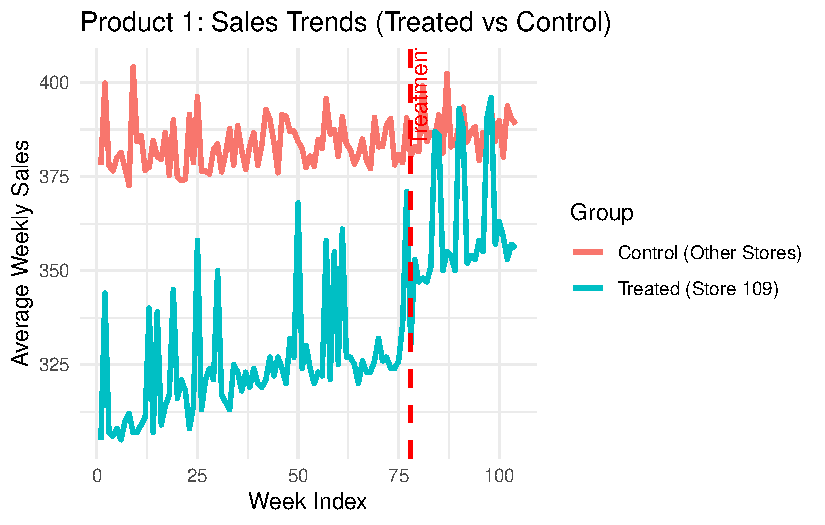
\includegraphics[keepaspectratio]{Portfolio_Task_4_files/figure-pdf/Visual inspection of parallel trends assumption-1.pdf}}

\begin{Shaded}
\begin{Highlighting}[]
\CommentTok{\# {-}{-}{-} Product 2 Plot {-}{-}{-}}
\NormalTok{trend\_data\_p2 }\OtherTok{\textless{}{-}}\NormalTok{ df }\SpecialCharTok{\%\textgreater{}\%}
  \FunctionTok{group\_by}\NormalTok{(Weekind, is\_treated\_store) }\SpecialCharTok{\%\textgreater{}\%}
  \FunctionTok{summarise}\NormalTok{(}\AttributeTok{mean\_sales =} \FunctionTok{mean}\NormalTok{(p2sales, }\AttributeTok{na.rm =} \ConstantTok{TRUE}\NormalTok{), }\AttributeTok{.groups =} \StringTok{\textquotesingle{}drop\textquotesingle{}}\NormalTok{) }\SpecialCharTok{\%\textgreater{}\%}
  \FunctionTok{mutate}\NormalTok{(}\AttributeTok{Group =} \FunctionTok{ifelse}\NormalTok{(is\_treated\_store }\SpecialCharTok{==} \DecValTok{1}\NormalTok{, }\StringTok{"Treated (Store 109)"}\NormalTok{, }\StringTok{"Control (Other Stores)"}\NormalTok{))}

\NormalTok{plot\_p2 }\OtherTok{\textless{}{-}} \FunctionTok{ggplot}\NormalTok{(trend\_data\_p2, }\FunctionTok{aes}\NormalTok{(}\AttributeTok{x =}\NormalTok{ Weekind, }\AttributeTok{y =}\NormalTok{ mean\_sales, }\AttributeTok{color =}\NormalTok{ Group)) }\SpecialCharTok{+}
  \FunctionTok{geom\_line}\NormalTok{(}\AttributeTok{linewidth =} \DecValTok{1}\NormalTok{) }\SpecialCharTok{+}
  \FunctionTok{geom\_vline}\NormalTok{(}\AttributeTok{xintercept =} \DecValTok{78}\NormalTok{, }\AttributeTok{linetype =} \StringTok{"dashed"}\NormalTok{, }\AttributeTok{color =} \StringTok{"red"}\NormalTok{, }\AttributeTok{linewidth =} \DecValTok{1}\NormalTok{) }\SpecialCharTok{+}
  \FunctionTok{annotate}\NormalTok{(}\StringTok{"text"}\NormalTok{, }\AttributeTok{x =} \DecValTok{76}\NormalTok{, }\AttributeTok{y =} \FunctionTok{max}\NormalTok{(trend\_data\_p2}\SpecialCharTok{$}\NormalTok{mean\_sales), }
           \AttributeTok{label =} \StringTok{"Treatment Start"}\NormalTok{, }\AttributeTok{angle =} \DecValTok{90}\NormalTok{, }\AttributeTok{vjust =} \FloatTok{1.5}\NormalTok{, }\AttributeTok{color =} \StringTok{"red"}\NormalTok{) }\SpecialCharTok{+}
  \FunctionTok{labs}\NormalTok{(}\AttributeTok{title =} \StringTok{"Product 2: Sales Trends (Treated vs Control)"}\NormalTok{,}
       \AttributeTok{x =} \StringTok{"Week Index"}\NormalTok{,}
       \AttributeTok{y =} \StringTok{"Average Weekly Sales"}\NormalTok{) }\SpecialCharTok{+}
  \FunctionTok{theme\_minimal}\NormalTok{()}

\FunctionTok{print}\NormalTok{(plot\_p2)}
\end{Highlighting}
\end{Shaded}

\pandocbounded{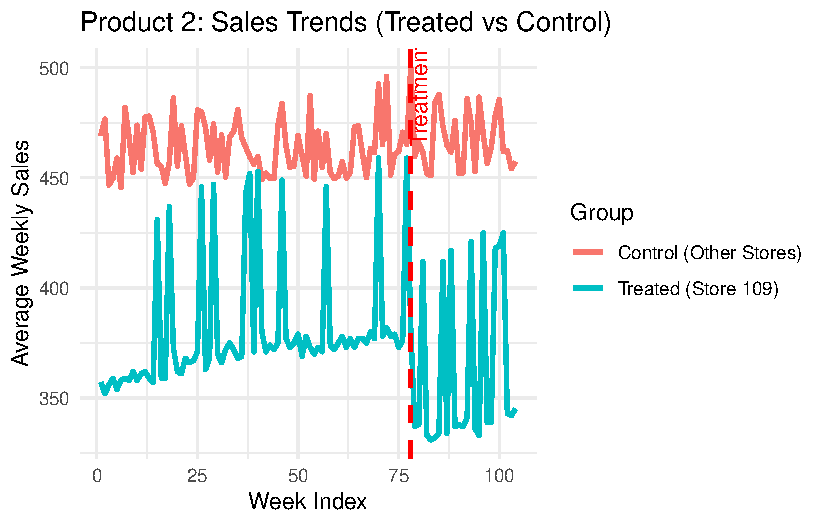
\includegraphics[keepaspectratio]{Portfolio_Task_4_files/figure-pdf/Visual inspection of parallel trends assumption-2.pdf}}

\subsubsection{Statistical test for parallel trends: Pre-treatment
interaction
model}\label{statistical-test-for-parallel-trends-pre-treatment-interaction-model}

Additionally to doing the visual inspection, we can also run a formal
statistical test for parallel trends by regressing sales on the store
dummy, a linear time trend (Weekind), and their interaction, but only
using the pre-treatment data (Weeks 1 to 77). If the coefficient on the
interaction term is statistically significant, it would suggest that the
treated store had a different trend compared to the control stores even
before the treatment started, which would violate the parallel trends
assumption and potentially bias our DiD and SDID estimates.

\begin{Shaded}
\begin{Highlighting}[]
\CommentTok{\# Filter the data to ONLY include the pre{-}treatment period (Weeks 1 to 77)}
\NormalTok{df\_pre }\OtherTok{\textless{}{-}}\NormalTok{ df }\SpecialCharTok{\%\textgreater{}\%} \FunctionTok{filter}\NormalTok{(Weekind }\SpecialCharTok{\textless{}} \DecValTok{78}\NormalTok{)}

\CommentTok{\# {-}{-}{-} Product 1: Parallel Trends Test {-}{-}{-}}
\NormalTok{pt\_test\_p1 }\OtherTok{\textless{}{-}} \FunctionTok{lm}\NormalTok{(p1sales }\SpecialCharTok{\textasciitilde{}}\NormalTok{ is\_treated\_store }\SpecialCharTok{*}\NormalTok{ Weekind, }\AttributeTok{data =}\NormalTok{ df\_pre)}
\FunctionTok{coeftest}\NormalTok{(pt\_test\_p1)[}\StringTok{"is\_treated\_store:Weekind"}\NormalTok{, , drop }\OtherTok{=} \ConstantTok{FALSE}\NormalTok{]}
\end{Highlighting}
\end{Shaded}

\begin{verbatim}
                          Estimate Std. Error   t value  Pr(>|t|)
is_treated_store:Weekind 0.2435446  0.3551978 0.6856591 0.4930266
\end{verbatim}

\begin{Shaded}
\begin{Highlighting}[]
\CommentTok{\# {-}{-}{-} Product 2: Parallel Trends Test {-}{-}{-}}
\NormalTok{pt\_test\_p2 }\OtherTok{\textless{}{-}} \FunctionTok{lm}\NormalTok{(p2sales }\SpecialCharTok{\textasciitilde{}}\NormalTok{ is\_treated\_store }\SpecialCharTok{*}\NormalTok{ Weekind, }\AttributeTok{data =}\NormalTok{ df\_pre)}
\FunctionTok{coeftest}\NormalTok{(pt\_test\_p2)[}\StringTok{"is\_treated\_store:Weekind"}\NormalTok{, , drop }\OtherTok{=} \ConstantTok{FALSE}\NormalTok{]}
\end{Highlighting}
\end{Shaded}

\begin{verbatim}
                          Estimate Std. Error   t value  Pr(>|t|)
is_treated_store:Weekind 0.3467782  0.5785286 0.5994142 0.5489809
\end{verbatim}

\textbf{Findings:} For both products, the visual interpretation leads to
believe that there is a slight positive trend in the treated store's
sales compared to the control stores in the pre-treatment period, which
could potentially violate the parallel trends assumption. However, the
formal statistical test for parallel trends (the interaction term
between the treated store dummy and the linear time trend
{[}is\_treated\_store:Weekind{]}) is not statistically significant for
either product (p \textgreater{} 0.05). This suggests that while there
may be some visual differences in trends, they are not statistically
significant enough to conclusively reject the parallel trends assumption
possibly due to limited sample size or high variability. Therefore, we
can proceed with our DiD and SDID analyses, but we should be cautious in
interpreting the results given the potential for some underlying
differences in pre-treatment trends.

\subsection{Evaluating the treatment effect using DiD, SC, and SDID
methods for each
product}\label{evaluating-the-treatment-effect-using-did-sc-and-sdid-methods-for-each-product}

\subsubsection{Product 1: p1sales}\label{product-1-p1sales}

\begin{Shaded}
\begin{Highlighting}[]
\CommentTok{\# Ensure data frame is standard class (synthdid prefers plain data.frames over tibbles)}
\NormalTok{df }\OtherTok{\textless{}{-}} \FunctionTok{as.data.frame}\NormalTok{(df)}

\CommentTok{\# Setup panel matrices for Product 1}
\NormalTok{setup\_p1 }\OtherTok{\textless{}{-}} \FunctionTok{panel.matrices}\NormalTok{(}
\NormalTok{  df,}
  \AttributeTok{unit =} \StringTok{"storeNum"}\NormalTok{,}
  \AttributeTok{time =} \StringTok{"Weekind"}\NormalTok{,}
  \AttributeTok{outcome =} \StringTok{"p1sales"}\NormalTok{,}
  \AttributeTok{treatment =} \StringTok{"treated"}
\NormalTok{)}

\CommentTok{\# Estimate the treatment effects for Product 1}
\NormalTok{sdid\_est\_p1 }\OtherTok{\textless{}{-}} \FunctionTok{synthdid\_estimate}\NormalTok{(setup\_p1}\SpecialCharTok{$}\NormalTok{Y, setup\_p1}\SpecialCharTok{$}\NormalTok{N0, setup\_p1}\SpecialCharTok{$}\NormalTok{T0)}
\NormalTok{did\_est\_p1 }\OtherTok{\textless{}{-}} \FunctionTok{did\_estimate}\NormalTok{(setup\_p1}\SpecialCharTok{$}\NormalTok{Y, setup\_p1}\SpecialCharTok{$}\NormalTok{N0, setup\_p1}\SpecialCharTok{$}\NormalTok{T0)}
\NormalTok{sc\_est\_p1 }\OtherTok{\textless{}{-}} \FunctionTok{sc\_estimate}\NormalTok{(setup\_p1}\SpecialCharTok{$}\NormalTok{Y, setup\_p1}\SpecialCharTok{$}\NormalTok{N0, setup\_p1}\SpecialCharTok{$}\NormalTok{T0)}
\NormalTok{estimates\_p1 }\OtherTok{=} \FunctionTok{list}\NormalTok{(did\_est\_p1, sc\_est\_p1, sdid\_est\_p1)}

\CommentTok{\# Print the estimates}
\FunctionTok{names}\NormalTok{(estimates\_p1) }\OtherTok{=} \FunctionTok{c}\NormalTok{(}\StringTok{\textquotesingle{}Diff{-}in{-}Diff\textquotesingle{}}\NormalTok{, }\StringTok{\textquotesingle{}Synthetic Control\textquotesingle{}}\NormalTok{, }\StringTok{\textquotesingle{}Synthetic Diff{-}in{-}Diff\textquotesingle{}}\NormalTok{)}
\FunctionTok{print}\NormalTok{(}\FunctionTok{unlist}\NormalTok{(estimates\_p1))}
\end{Highlighting}
\end{Shaded}

\begin{verbatim}
          Diff-in-Diff      Synthetic Control Synthetic Diff-in-Diff 
              32.21775               36.37194               14.88871 
\end{verbatim}

\begin{Shaded}
\begin{Highlighting}[]
\CommentTok{\# Plot 1: Trends of treated vs. synthetic control}
\FunctionTok{synthdid\_plot}\NormalTok{(estimates\_p1, }\AttributeTok{facet.vertical =} \ConstantTok{FALSE}\NormalTok{)}
\end{Highlighting}
\end{Shaded}

\pandocbounded{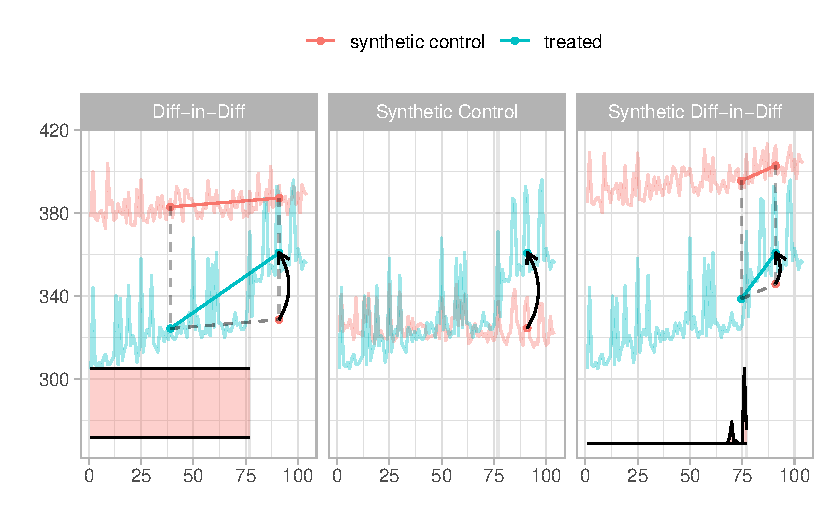
\includegraphics[keepaspectratio]{Portfolio_Task_4_files/figure-pdf/DiD, SC, and SDID analyses for Product 1-1.pdf}}

\begin{Shaded}
\begin{Highlighting}[]
\CommentTok{\# Plot 2: See which control stores received the highest weights}
\FunctionTok{synthdid\_units\_plot}\NormalTok{(estimates\_p1)}
\end{Highlighting}
\end{Shaded}

\pandocbounded{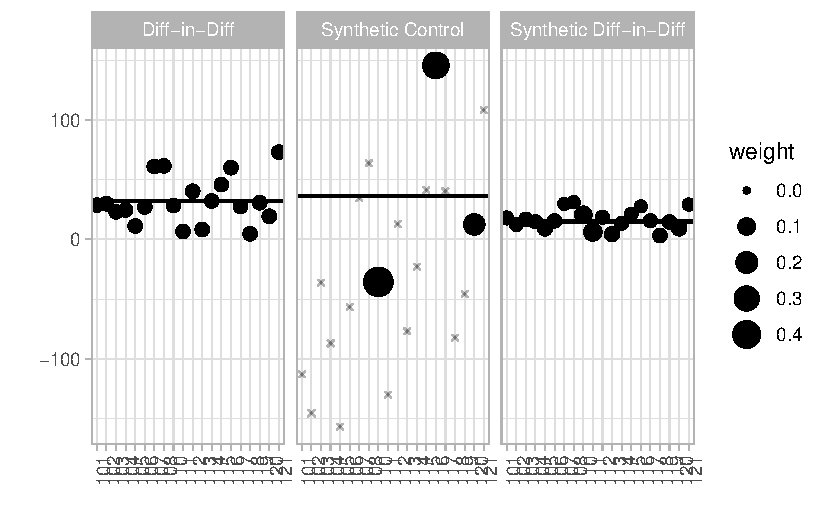
\includegraphics[keepaspectratio]{Portfolio_Task_4_files/figure-pdf/DiD, SC, and SDID analyses for Product 1-2.pdf}}

\subsubsection{Product 2: p2sales}\label{product-2-p2sales}

The same steps as for Product 1 are repeated for Product 2.

\begin{Shaded}
\begin{Highlighting}[]
\CommentTok{\# Setup panel matrices for Product 2}
\NormalTok{setup\_p2 }\OtherTok{\textless{}{-}} \FunctionTok{panel.matrices}\NormalTok{(}
\NormalTok{  df,}
  \AttributeTok{unit =} \StringTok{"storeNum"}\NormalTok{,}
  \AttributeTok{time =} \StringTok{"Weekind"}\NormalTok{,}
  \AttributeTok{outcome =} \StringTok{"p2sales"}\NormalTok{,}
  \AttributeTok{treatment =} \StringTok{"treated"}
\NormalTok{)}

\CommentTok{\# Estimate the treatment effects for Product 2}
\NormalTok{sdid\_est\_p2 }\OtherTok{\textless{}{-}} \FunctionTok{synthdid\_estimate}\NormalTok{(setup\_p2}\SpecialCharTok{$}\NormalTok{Y, setup\_p2}\SpecialCharTok{$}\NormalTok{N0, setup\_p2}\SpecialCharTok{$}\NormalTok{T0)}
\NormalTok{did\_est\_p2 }\OtherTok{\textless{}{-}} \FunctionTok{did\_estimate}\NormalTok{(setup\_p2}\SpecialCharTok{$}\NormalTok{Y, setup\_p2}\SpecialCharTok{$}\NormalTok{N0, setup\_p2}\SpecialCharTok{$}\NormalTok{T0)}
\NormalTok{sc\_est\_p2 }\OtherTok{\textless{}{-}} \FunctionTok{sc\_estimate}\NormalTok{(setup\_p2}\SpecialCharTok{$}\NormalTok{Y, setup\_p2}\SpecialCharTok{$}\NormalTok{N0, setup\_p2}\SpecialCharTok{$}\NormalTok{T0)}
\NormalTok{estimates\_p2 }\OtherTok{=} \FunctionTok{list}\NormalTok{(did\_est\_p2, sc\_est\_p2, sdid\_est\_p2)}

\CommentTok{\# Print the estimates}
\FunctionTok{names}\NormalTok{(estimates\_p2) }\OtherTok{=} \FunctionTok{c}\NormalTok{(}\StringTok{\textquotesingle{}Diff{-}in{-}Diff\textquotesingle{}}\NormalTok{, }\StringTok{\textquotesingle{}Synthetic Control\textquotesingle{}}\NormalTok{, }\StringTok{\textquotesingle{}Synthetic Diff{-}in{-}Diff\textquotesingle{}}\NormalTok{)}
\FunctionTok{print}\NormalTok{(}\FunctionTok{unlist}\NormalTok{(estimates\_p2))}
\end{Highlighting}
\end{Shaded}

\begin{verbatim}
          Diff-in-Diff      Synthetic Control Synthetic Diff-in-Diff 
             -22.25818              -25.97635              -42.64470 
\end{verbatim}

\begin{Shaded}
\begin{Highlighting}[]
\CommentTok{\# Plot 1: Trends of treated vs. synthetic control}
\FunctionTok{synthdid\_plot}\NormalTok{(estimates\_p2, }\AttributeTok{facet.vertical =} \ConstantTok{FALSE}\NormalTok{)}
\end{Highlighting}
\end{Shaded}

\pandocbounded{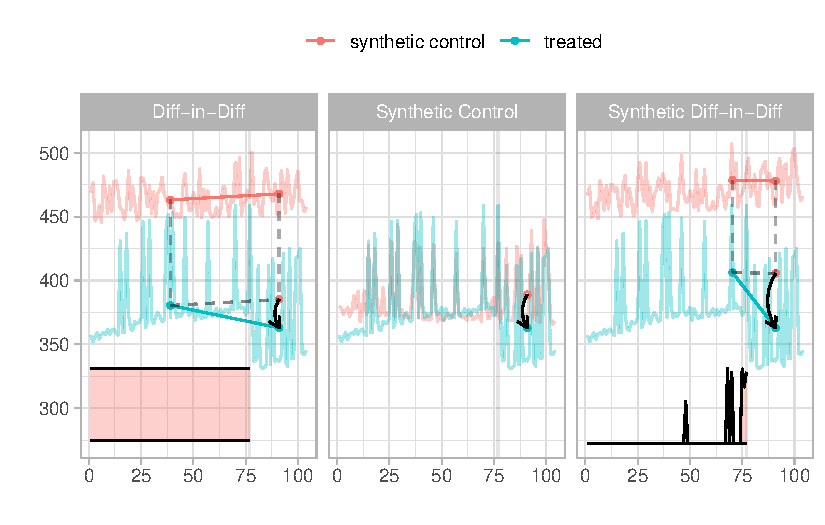
\includegraphics[keepaspectratio]{Portfolio_Task_4_files/figure-pdf/DiD, SC, and SDID analyses for Product 2-1.pdf}}

\begin{Shaded}
\begin{Highlighting}[]
\CommentTok{\# Plot 2: See which control stores received the highest weights}
\FunctionTok{synthdid\_units\_plot}\NormalTok{(estimates\_p2)}
\end{Highlighting}
\end{Shaded}

\pandocbounded{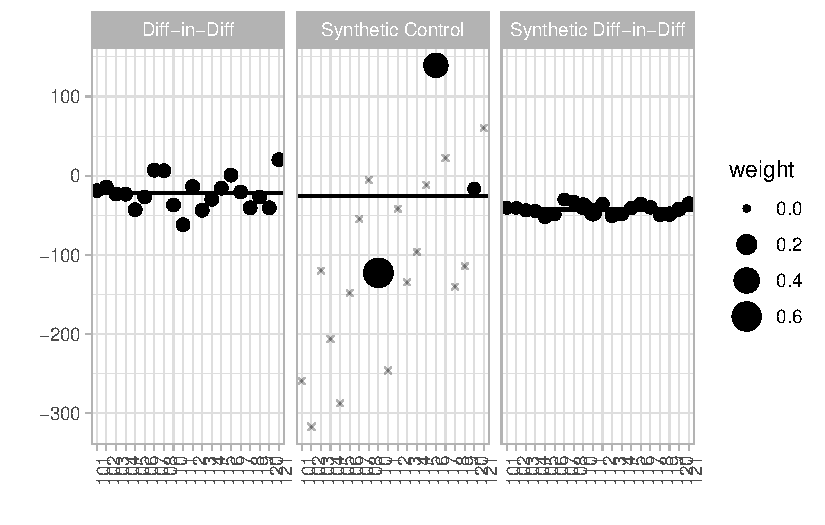
\includegraphics[keepaspectratio]{Portfolio_Task_4_files/figure-pdf/DiD, SC, and SDID analyses for Product 2-2.pdf}}

\subsubsection{SC diagnostics: Pre/Post RMSPE and donor
weights}\label{sc-diagnostics-prepost-rmspe-and-donor-weights}

The two tables below report the standard SC diagnostics. Pre-RMSPE
measures how well the synthetic control matches the treated store before
the treatment (small values mean a good pre-treatment fit), and
Post-RMSPE measures the gap after the treatment (a larger Post-RMSPE
relative to Pre-RMSPE is the SC signature for a real treatment effect).
The donor-weight tables make the synthetic match explicit by listing
which control stores carry non-trivial weight in the SC estimator for
each product.

\begin{Shaded}
\begin{Highlighting}[]
\CommentTok{\# Helper: extract synthetic counterfactual + RMSPE + donor weights from an SC estimate}
\NormalTok{sc\_diagnostics }\OtherTok{\textless{}{-}} \ControlFlowTok{function}\NormalTok{(sc\_est, setup) \{}
\NormalTok{  Y  }\OtherTok{\textless{}{-}}\NormalTok{ setup}\SpecialCharTok{$}\NormalTok{Y}
\NormalTok{  N0 }\OtherTok{\textless{}{-}}\NormalTok{ setup}\SpecialCharTok{$}\NormalTok{N0}
\NormalTok{  T0 }\OtherTok{\textless{}{-}}\NormalTok{ setup}\SpecialCharTok{$}\NormalTok{T0}
\NormalTok{  N  }\OtherTok{\textless{}{-}} \FunctionTok{nrow}\NormalTok{(Y)}
\NormalTok{  T\_ }\OtherTok{\textless{}{-}} \FunctionTok{ncol}\NormalTok{(Y)}

  \CommentTok{\# SC donor weights (length N0): synthetic counterfactual is weighted avg of controls}
\NormalTok{  omega }\OtherTok{\textless{}{-}} \FunctionTok{attr}\NormalTok{(sc\_est, }\StringTok{"weights"}\NormalTok{)}\SpecialCharTok{$}\NormalTok{omega}

  \CommentTok{\# Synthetic counterfactual time series for the treated unit}
\NormalTok{  y\_synth }\OtherTok{\textless{}{-}} \FunctionTok{as.vector}\NormalTok{(}\FunctionTok{t}\NormalTok{(omega) }\SpecialCharTok{\%*\%}\NormalTok{ Y[}\DecValTok{1}\SpecialCharTok{:}\NormalTok{N0, , }\AttributeTok{drop =} \ConstantTok{FALSE}\NormalTok{])}
\NormalTok{  y\_treat }\OtherTok{\textless{}{-}} \FunctionTok{as.vector}\NormalTok{(Y[N, ])  }\CommentTok{\# single treated unit at the bottom}

\NormalTok{  pre\_rmspe  }\OtherTok{\textless{}{-}} \FunctionTok{sqrt}\NormalTok{(}\FunctionTok{mean}\NormalTok{((y\_treat[}\DecValTok{1}\SpecialCharTok{:}\NormalTok{T0]          }\SpecialCharTok{{-}}\NormalTok{ y\_synth[}\DecValTok{1}\SpecialCharTok{:}\NormalTok{T0])}\SpecialCharTok{\^{}}\DecValTok{2}\NormalTok{))}
\NormalTok{  post\_rmspe }\OtherTok{\textless{}{-}} \FunctionTok{sqrt}\NormalTok{(}\FunctionTok{mean}\NormalTok{((y\_treat[(T0}\SpecialCharTok{+}\DecValTok{1}\NormalTok{)}\SpecialCharTok{:}\NormalTok{T\_]     }\SpecialCharTok{{-}}\NormalTok{ y\_synth[(T0}\SpecialCharTok{+}\DecValTok{1}\NormalTok{)}\SpecialCharTok{:}\NormalTok{T\_])}\SpecialCharTok{\^{}}\DecValTok{2}\NormalTok{))}

\NormalTok{  donor\_ids }\OtherTok{\textless{}{-}} \FunctionTok{rownames}\NormalTok{(Y)[}\DecValTok{1}\SpecialCharTok{:}\NormalTok{N0]}
\NormalTok{  donor\_w   }\OtherTok{\textless{}{-}} \FunctionTok{data.frame}\NormalTok{(}\AttributeTok{Store =}\NormalTok{ donor\_ids, }\AttributeTok{Weight =} \FunctionTok{round}\NormalTok{(omega, }\DecValTok{4}\NormalTok{),}
                          \AttributeTok{row.names =} \ConstantTok{NULL}\NormalTok{)}
\NormalTok{  donor\_w   }\OtherTok{\textless{}{-}}\NormalTok{ donor\_w[}\FunctionTok{order}\NormalTok{(}\SpecialCharTok{{-}}\NormalTok{donor\_w}\SpecialCharTok{$}\NormalTok{Weight), ]}

  \FunctionTok{list}\NormalTok{(}\AttributeTok{pre =}\NormalTok{ pre\_rmspe, }\AttributeTok{post =}\NormalTok{ post\_rmspe, }\AttributeTok{donors =}\NormalTok{ donor\_w)}
\NormalTok{\}}

\NormalTok{diag\_p1 }\OtherTok{\textless{}{-}} \FunctionTok{sc\_diagnostics}\NormalTok{(sc\_est\_p1, setup\_p1)}
\NormalTok{diag\_p2 }\OtherTok{\textless{}{-}} \FunctionTok{sc\_diagnostics}\NormalTok{(sc\_est\_p2, setup\_p2)}

\CommentTok{\# Pre/Post RMSPE table}
\NormalTok{rmspe\_table }\OtherTok{\textless{}{-}} \FunctionTok{data.frame}\NormalTok{(}
  \AttributeTok{Period =} \FunctionTok{c}\NormalTok{(}\StringTok{"Pre{-}treatment RMSPE"}\NormalTok{, }\StringTok{"Post{-}treatment RMSPE"}\NormalTok{),}
  \AttributeTok{Product\_1 =} \FunctionTok{c}\NormalTok{(}\FunctionTok{round}\NormalTok{(diag\_p1}\SpecialCharTok{$}\NormalTok{pre, }\DecValTok{3}\NormalTok{), }\FunctionTok{round}\NormalTok{(diag\_p1}\SpecialCharTok{$}\NormalTok{post, }\DecValTok{3}\NormalTok{)),}
  \AttributeTok{Product\_2 =} \FunctionTok{c}\NormalTok{(}\FunctionTok{round}\NormalTok{(diag\_p2}\SpecialCharTok{$}\NormalTok{pre, }\DecValTok{3}\NormalTok{), }\FunctionTok{round}\NormalTok{(diag\_p2}\SpecialCharTok{$}\NormalTok{post, }\DecValTok{3}\NormalTok{))}
\NormalTok{)}

\FunctionTok{kable}\NormalTok{(rmspe\_table,}
      \AttributeTok{col.names =} \FunctionTok{c}\NormalTok{(}\StringTok{""}\NormalTok{, }\StringTok{"Product 1"}\NormalTok{, }\StringTok{"Product 2"}\NormalTok{),}
      \AttributeTok{caption =} \StringTok{"Synthetic Control: pre/post RMSPE"}\NormalTok{,}
      \AttributeTok{align =} \FunctionTok{c}\NormalTok{(}\StringTok{"l"}\NormalTok{, }\StringTok{"c"}\NormalTok{, }\StringTok{"c"}\NormalTok{))}
\end{Highlighting}
\end{Shaded}

\begin{longtable}[]{@{}lcc@{}}
\caption{Synthetic Control: pre/post RMSPE}\tabularnewline
\toprule\noalign{}
& Product 1 & Product 2 \\
\midrule\noalign{}
\endfirsthead
\toprule\noalign{}
& Product 1 & Product 2 \\
\midrule\noalign{}
\endhead
\bottomrule\noalign{}
\endlastfoot
Pre-treatment RMSPE & 11.092 & 14.442 \\
Post-treatment RMSPE & 38.088 & 30.632 \\
\end{longtable}

\begin{Shaded}
\begin{Highlighting}[]
\CommentTok{\# Donor weights — keep only stores with non{-}trivial weight (\textgreater{}0.01) for readability}
\NormalTok{donors\_p1 }\OtherTok{\textless{}{-}}\NormalTok{ diag\_p1}\SpecialCharTok{$}\NormalTok{donors[diag\_p1}\SpecialCharTok{$}\NormalTok{donors}\SpecialCharTok{$}\NormalTok{Weight }\SpecialCharTok{\textgreater{}} \FloatTok{0.01}\NormalTok{, ]}
\NormalTok{donors\_p2 }\OtherTok{\textless{}{-}}\NormalTok{ diag\_p2}\SpecialCharTok{$}\NormalTok{donors[diag\_p2}\SpecialCharTok{$}\NormalTok{donors}\SpecialCharTok{$}\NormalTok{Weight }\SpecialCharTok{\textgreater{}} \FloatTok{0.01}\NormalTok{, ]}

\FunctionTok{kable}\NormalTok{(donors\_p1,}
      \AttributeTok{caption =} \StringTok{"Synthetic Control donor weights — Product 1 (stores with weight \textgreater{} 0.01)"}\NormalTok{,}
      \AttributeTok{align =} \FunctionTok{c}\NormalTok{(}\StringTok{"l"}\NormalTok{, }\StringTok{"c"}\NormalTok{),}
      \AttributeTok{row.names =} \ConstantTok{FALSE}\NormalTok{)}
\end{Highlighting}
\end{Shaded}

\begin{longtable}[]{@{}lc@{}}
\caption{Synthetic Control donor weights --- Product 1 (stores with
weight \textgreater{} 0.01)}\tabularnewline
\toprule\noalign{}
Store & Weight \\
\midrule\noalign{}
\endfirsthead
\toprule\noalign{}
Store & Weight \\
\midrule\noalign{}
\endhead
\bottomrule\noalign{}
\endlastfoot
110 & 0.4614 \\
116 & 0.3468 \\
120 & 0.1907 \\
\end{longtable}

\begin{Shaded}
\begin{Highlighting}[]
\FunctionTok{kable}\NormalTok{(donors\_p2,}
      \AttributeTok{caption =} \StringTok{"Synthetic Control donor weights — Product 2 (stores with weight \textgreater{} 0.01)"}\NormalTok{,}
      \AttributeTok{align =} \FunctionTok{c}\NormalTok{(}\StringTok{"l"}\NormalTok{, }\StringTok{"c"}\NormalTok{),}
      \AttributeTok{row.names =} \ConstantTok{FALSE}\NormalTok{)}
\end{Highlighting}
\end{Shaded}

\begin{longtable}[]{@{}lc@{}}
\caption{Synthetic Control donor weights --- Product 2 (stores with
weight \textgreater{} 0.01)}\tabularnewline
\toprule\noalign{}
Store & Weight \\
\midrule\noalign{}
\endfirsthead
\toprule\noalign{}
Store & Weight \\
\midrule\noalign{}
\endhead
\bottomrule\noalign{}
\endlastfoot
110 & 0.6078 \\
116 & 0.3548 \\
120 & 0.0365 \\
\end{longtable}

\section{Expensions to the analysis}\label{expensions-to-the-analysis}

Two possible expansions to the analysis include:

\begin{enumerate}
\def\labelenumi{\arabic{enumi}.}
\tightlist
\item
  Running the same DiD interaction estimated via pooled OLS rather than
  within-transformation, with the full covariate set added explicitly.
  This estimates the same DiD effect --- the coefficient on the treated
  × post interaction --- and lets us see how much of the store-level
  variation the covariate set captures relative to the TWFE
  specification (the brief's ``panel DID'').
\item
  Implementing a version of the SDID method that first regresses out the
  effects of price and promotions (using the Frisch-Waugh-Lovell
  theorem) before applying the SDID estimator to the residuals. This
  will allow us to see how controlling for these covariates in a more
  flexible way (without assuming linearity or additivity) affects the
  estimates and their precision.
\end{enumerate}

\subsection{Pooled DiD with
covariates}\label{pooled-did-with-covariates}

This is the same DiD effect estimated via pooled OLS rather than
within-transformation:
\(Y_{it} = \alpha + \gamma\, T_i + \lambda\, POST_t + \delta\, (T_i \cdot POST_t) + X\beta + \varepsilon_{it}\),
with \texttt{treated} as the interaction term. With explicit covariates
instead of fixed effects, we can see how much of the store-level
variation the covariate set captures relative to TWFE --- useful for
judging whether the included covariates do the work fixed effects would
otherwise do. The brief's ``panel DID'' is the TWFE specification above;
this pooled-OLS form is the canonical Regression DiD (Angrist \& Pischke
2009, Ch. 5; lecture 11) augmented with covariates.

\subsubsection{Product 1: Pooled DiD with
covariates}\label{product-1-pooled-did-with-covariates}

\begin{Shaded}
\begin{Highlighting}[]
\NormalTok{did\_cov\_p1 }\OtherTok{\textless{}{-}} \FunctionTok{plm}\NormalTok{(p1sales }\SpecialCharTok{\textasciitilde{}}\NormalTok{ is\_treated\_store }\SpecialCharTok{+}\NormalTok{ post\_treatment }\SpecialCharTok{+}\NormalTok{ treated }\SpecialCharTok{+}
\NormalTok{                            p1price }\SpecialCharTok{+}\NormalTok{ p1prom }\SpecialCharTok{+}\NormalTok{ compind }\SpecialCharTok{+}\NormalTok{ storesize }\SpecialCharTok{+}\NormalTok{ citysize,}
                  \AttributeTok{data =}\NormalTok{ pdf,}
                  \AttributeTok{model =} \StringTok{"pooling"}\NormalTok{)}
\FunctionTok{coeftest}\NormalTok{(did\_cov\_p1)[}\StringTok{"treated"}\NormalTok{, , drop }\OtherTok{=} \ConstantTok{FALSE}\NormalTok{]}
\end{Highlighting}
\end{Shaded}

\begin{verbatim}
        Estimate Std. Error  t value     Pr(>|t|)
treated 29.97353   2.528654 11.85355 1.874956e-31
\end{verbatim}

\begin{Shaded}
\begin{Highlighting}[]
\CommentTok{\# Product 1: Pooled DiD with Clustered Standard Errors (treatment row)}
\FunctionTok{coeftest}\NormalTok{(did\_cov\_p1, }\AttributeTok{vcov =} \FunctionTok{vcovHC}\NormalTok{(did\_cov\_p1, }\AttributeTok{type =} \StringTok{"HC1"}\NormalTok{, }\AttributeTok{cluster =} \StringTok{"group"}\NormalTok{))[}\StringTok{"treated"}\NormalTok{, , drop }\OtherTok{=} \ConstantTok{FALSE}\NormalTok{]}
\end{Highlighting}
\end{Shaded}

\begin{verbatim}
        Estimate Std. Error  t value     Pr(>|t|)
treated 29.97353   4.039648 7.419837 1.672423e-13
\end{verbatim}

\subsubsection{Product 2: Pooled DiD with
covariates}\label{product-2-pooled-did-with-covariates}

\begin{Shaded}
\begin{Highlighting}[]
\NormalTok{did\_cov\_p2 }\OtherTok{\textless{}{-}} \FunctionTok{plm}\NormalTok{(p2sales }\SpecialCharTok{\textasciitilde{}}\NormalTok{ is\_treated\_store }\SpecialCharTok{+}\NormalTok{ post\_treatment }\SpecialCharTok{+}\NormalTok{ treated }\SpecialCharTok{+}
\NormalTok{                            p2price }\SpecialCharTok{+}\NormalTok{ p2prom }\SpecialCharTok{+}\NormalTok{ compind }\SpecialCharTok{+}\NormalTok{ storesize }\SpecialCharTok{+}\NormalTok{ citysize,}
                  \AttributeTok{data =}\NormalTok{ pdf,}
                  \AttributeTok{model =} \StringTok{"pooling"}\NormalTok{)}
\FunctionTok{coeftest}\NormalTok{(did\_cov\_p2)[}\StringTok{"treated"}\NormalTok{, , drop }\OtherTok{=} \ConstantTok{FALSE}\NormalTok{]}
\end{Highlighting}
\end{Shaded}

\begin{verbatim}
         Estimate Std. Error   t value     Pr(>|t|)
treated -34.35383   3.060016 -11.22668 1.799889e-28
\end{verbatim}

\begin{Shaded}
\begin{Highlighting}[]
\CommentTok{\# Product 2: Pooled DiD with Clustered Standard Errors (treatment row)}
\FunctionTok{coeftest}\NormalTok{(did\_cov\_p2, }\AttributeTok{vcov =} \FunctionTok{vcovHC}\NormalTok{(did\_cov\_p2, }\AttributeTok{type =} \StringTok{"HC1"}\NormalTok{, }\AttributeTok{cluster =} \StringTok{"group"}\NormalTok{))[}\StringTok{"treated"}\NormalTok{, , drop }\OtherTok{=} \ConstantTok{FALSE}\NormalTok{]}
\end{Highlighting}
\end{Shaded}

\begin{verbatim}
         Estimate Std. Error   t value     Pr(>|t|)
treated -34.35383   4.460595 -7.701624 2.025479e-14
\end{verbatim}

\subsection{Synthetic DiD regressing out the
covariates}\label{synthetic-did-regressing-out-the-covariates}

Given that the base synthdid package used does not easily accept
additional control variables (like price and promotions) directly into
its primary matrix setup, we can implement a solution based on the
Frisch-Waugh-Lovell (FWL) theorem: we first use a linear regression to
predict sales based only on the covariates, extract the residuals (the
portion of sales unexplained by price, promotions, etc.), and then apply
the SDID model to those residuals.

By adding the overall mean back to the residuals, we keep the
interpretation on the same scale as the original sales volume.

\subsubsection{Product 1: p1sales}\label{product-1-p1sales-1}

\begin{Shaded}
\begin{Highlighting}[]
\CommentTok{\# Run a linear model and extract the residuals (unexplained sales)}
\NormalTok{model\_p1 }\OtherTok{\textless{}{-}} \FunctionTok{lm}\NormalTok{(p1sales }\SpecialCharTok{\textasciitilde{}}\NormalTok{ p1price }\SpecialCharTok{+}\NormalTok{ p1prom }\SpecialCharTok{+}\NormalTok{ compind }\SpecialCharTok{+}\NormalTok{ storesize }\SpecialCharTok{+}\NormalTok{ citysize, }\AttributeTok{data =}\NormalTok{ df)}
\NormalTok{df}\SpecialCharTok{$}\NormalTok{p1sales\_adj }\OtherTok{\textless{}{-}} \FunctionTok{residuals}\NormalTok{(model\_p1) }\SpecialCharTok{+} \FunctionTok{mean}\NormalTok{(df}\SpecialCharTok{$}\NormalTok{p1sales, }\AttributeTok{na.rm =} \ConstantTok{TRUE}\NormalTok{)}

\CommentTok{\# Setup panel matrices using the NEW adjusted outcome variable}
\NormalTok{setup\_p1\_adj }\OtherTok{\textless{}{-}} \FunctionTok{panel.matrices}\NormalTok{(}
\NormalTok{  df,}
  \AttributeTok{unit =} \StringTok{"storeNum"}\NormalTok{,}
  \AttributeTok{time =} \StringTok{"Weekind"}\NormalTok{,}
  \AttributeTok{outcome =} \StringTok{"p1sales\_adj"}\NormalTok{, }
  \AttributeTok{treatment =} \StringTok{"treated"}
\NormalTok{)}

\CommentTok{\# Estimate the adjusted SDID Treatment Effect}
\NormalTok{sdid\_est\_p1\_adj }\OtherTok{\textless{}{-}} \FunctionTok{synthdid\_estimate}\NormalTok{(setup\_p1\_adj}\SpecialCharTok{$}\NormalTok{Y, setup\_p1\_adj}\SpecialCharTok{$}\NormalTok{N0, setup\_p1\_adj}\SpecialCharTok{$}\NormalTok{T0)}
\FunctionTok{print}\NormalTok{(sdid\_est\_p1\_adj)}
\end{Highlighting}
\end{Shaded}

\begin{verbatim}
synthdid: 18.519 +- NA. Effective N0/N0 = 14.1/20~0.7. Effective T0/T0 = 1.6/77~0.0. N1,T1 = 1,27. 
\end{verbatim}

\begin{Shaded}
\begin{Highlighting}[]
\CommentTok{\# Calculate and print confidence intervals for Product 1}
\NormalTok{se\_p1\_adj }\OtherTok{\textless{}{-}} \FunctionTok{sqrt}\NormalTok{(}\FunctionTok{vcov}\NormalTok{(sdid\_est\_p1\_adj, }\AttributeTok{method =} \StringTok{"placebo"}\NormalTok{))}
\FunctionTok{cat}\NormalTok{(}\FunctionTok{sprintf}\NormalTok{(}\StringTok{"Adjusted 95\%\% CI: [\%.2f, \%.2f]}\SpecialCharTok{\textbackslash{}n\textbackslash{}n}\StringTok{"}\NormalTok{, }
\NormalTok{            sdid\_est\_p1\_adj }\SpecialCharTok{{-}} \FloatTok{1.96} \SpecialCharTok{*}\NormalTok{ se\_p1\_adj, }
\NormalTok{            sdid\_est\_p1\_adj }\SpecialCharTok{+} \FloatTok{1.96} \SpecialCharTok{*}\NormalTok{ se\_p1\_adj))}
\end{Highlighting}
\end{Shaded}

\begin{verbatim}
Adjusted 95% CI: [12.04, 25.00]
\end{verbatim}

\begin{Shaded}
\begin{Highlighting}[]
\CommentTok{\# Visualize adjusted trends}
\FunctionTok{plot}\NormalTok{(sdid\_est\_p1\_adj) }\SpecialCharTok{+} \FunctionTok{theme\_minimal}\NormalTok{() }\SpecialCharTok{+} \FunctionTok{ylab}\NormalTok{(}\StringTok{"residual sales + grand mean"}\NormalTok{)}
\end{Highlighting}
\end{Shaded}

\pandocbounded{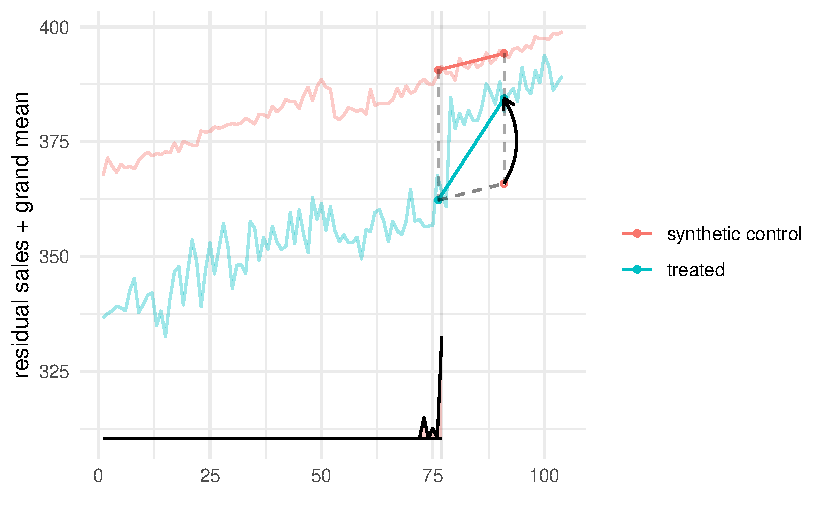
\includegraphics[keepaspectratio]{Portfolio_Task_4_files/figure-pdf/Regressing out covariates for Product 1-1.pdf}}

\subsubsection{Product 2: p2sales}\label{product-2-p2sales-1}

\begin{Shaded}
\begin{Highlighting}[]
\CommentTok{\# Run a linear model and extract the residuals (unexplained sales)}
\NormalTok{model\_p2 }\OtherTok{\textless{}{-}} \FunctionTok{lm}\NormalTok{(p2sales }\SpecialCharTok{\textasciitilde{}}\NormalTok{ p2price }\SpecialCharTok{+}\NormalTok{ p2prom }\SpecialCharTok{+}\NormalTok{ compind }\SpecialCharTok{+}\NormalTok{ storesize }\SpecialCharTok{+}\NormalTok{ citysize, }\AttributeTok{data =}\NormalTok{ df)}
\NormalTok{df}\SpecialCharTok{$}\NormalTok{p2sales\_adj }\OtherTok{\textless{}{-}} \FunctionTok{residuals}\NormalTok{(model\_p2) }\SpecialCharTok{+} \FunctionTok{mean}\NormalTok{(df}\SpecialCharTok{$}\NormalTok{p2sales, }\AttributeTok{na.rm =} \ConstantTok{TRUE}\NormalTok{)}

\CommentTok{\# Setup panel matrices using the NEW adjusted outcome variable}
\NormalTok{setup\_p2\_adj }\OtherTok{\textless{}{-}} \FunctionTok{panel.matrices}\NormalTok{(}
\NormalTok{  df,}
  \AttributeTok{unit =} \StringTok{"storeNum"}\NormalTok{,}
  \AttributeTok{time =} \StringTok{"Weekind"}\NormalTok{,}
  \AttributeTok{outcome =} \StringTok{"p2sales\_adj"}\NormalTok{, }
  \AttributeTok{treatment =} \StringTok{"treated"}
\NormalTok{)}

\CommentTok{\# Estimate the adjusted SDID Treatment Effect}
\NormalTok{sdid\_est\_p2\_adj }\OtherTok{\textless{}{-}} \FunctionTok{synthdid\_estimate}\NormalTok{(setup\_p2\_adj}\SpecialCharTok{$}\NormalTok{Y, setup\_p2\_adj}\SpecialCharTok{$}\NormalTok{N0, setup\_p2\_adj}\SpecialCharTok{$}\NormalTok{T0)}
\FunctionTok{print}\NormalTok{(sdid\_est\_p2\_adj)}
\end{Highlighting}
\end{Shaded}

\begin{verbatim}
synthdid: -42.649 +- NA. Effective N0/N0 = 16.2/20~0.8. Effective T0/T0 = 4.2/77~0.1. N1,T1 = 1,27. 
\end{verbatim}

\begin{Shaded}
\begin{Highlighting}[]
\CommentTok{\# Calculate and print confidence intervals for Product 2}
\NormalTok{se\_p2\_adj }\OtherTok{\textless{}{-}} \FunctionTok{sqrt}\NormalTok{(}\FunctionTok{vcov}\NormalTok{(sdid\_est\_p2\_adj, }\AttributeTok{method =} \StringTok{"placebo"}\NormalTok{))}
\FunctionTok{cat}\NormalTok{(}\FunctionTok{sprintf}\NormalTok{(}\StringTok{"Adjusted 95\%\% CI: [\%.2f, \%.2f]}\SpecialCharTok{\textbackslash{}n\textbackslash{}n}\StringTok{"}\NormalTok{, }
\NormalTok{            sdid\_est\_p2\_adj }\SpecialCharTok{{-}} \FloatTok{1.96} \SpecialCharTok{*}\NormalTok{ se\_p2\_adj, }
\NormalTok{            sdid\_est\_p2\_adj }\SpecialCharTok{+} \FloatTok{1.96} \SpecialCharTok{*}\NormalTok{ se\_p2\_adj))}
\end{Highlighting}
\end{Shaded}

\begin{verbatim}
Adjusted 95% CI: [-55.15, -30.14]
\end{verbatim}

\begin{Shaded}
\begin{Highlighting}[]
\CommentTok{\# Visualize adjusted trends}
\FunctionTok{plot}\NormalTok{(sdid\_est\_p2\_adj) }\SpecialCharTok{+} \FunctionTok{theme\_minimal}\NormalTok{() }\SpecialCharTok{+} \FunctionTok{ylab}\NormalTok{(}\StringTok{"residual sales + grand mean"}\NormalTok{)}
\end{Highlighting}
\end{Shaded}

\pandocbounded{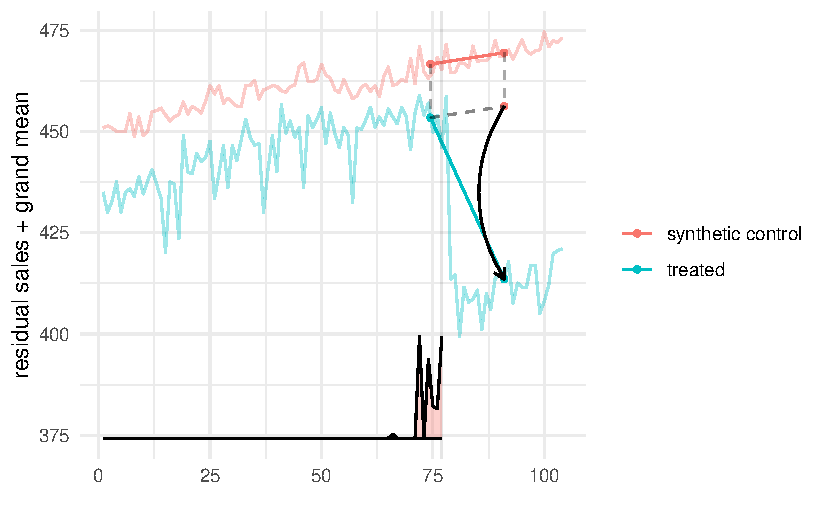
\includegraphics[keepaspectratio]{Portfolio_Task_4_files/figure-pdf/Regressing out covariates for Product 2-1.pdf}}

\section{Summary of Findings}\label{summary-of-findings}

\begin{longtable}[]{@{}
  >{\raggedright\arraybackslash}p{(\linewidth - 8\tabcolsep) * \real{0.4444}}
  >{\centering\arraybackslash}p{(\linewidth - 8\tabcolsep) * \real{0.1806}}
  >{\centering\arraybackslash}p{(\linewidth - 8\tabcolsep) * \real{0.0972}}
  >{\centering\arraybackslash}p{(\linewidth - 8\tabcolsep) * \real{0.1806}}
  >{\centering\arraybackslash}p{(\linewidth - 8\tabcolsep) * \real{0.0972}}@{}}
\caption{Comparison of Treatment Effect Estimates for Product 1 and
Product 2}\tabularnewline
\toprule\noalign{}
\begin{minipage}[b]{\linewidth}\raggedright
Model
\end{minipage} & \begin{minipage}[b]{\linewidth}\centering
P1 Estimate
\end{minipage} & \begin{minipage}[b]{\linewidth}\centering
P1 SE
\end{minipage} & \begin{minipage}[b]{\linewidth}\centering
P2 Estimate
\end{minipage} & \begin{minipage}[b]{\linewidth}\centering
P2 SE
\end{minipage} \\
\midrule\noalign{}
\endfirsthead
\toprule\noalign{}
\begin{minipage}[b]{\linewidth}\raggedright
Model
\end{minipage} & \begin{minipage}[b]{\linewidth}\centering
P1 Estimate
\end{minipage} & \begin{minipage}[b]{\linewidth}\centering
P1 SE
\end{minipage} & \begin{minipage}[b]{\linewidth}\centering
P2 Estimate
\end{minipage} & \begin{minipage}[b]{\linewidth}\centering
P2 SE
\end{minipage} \\
\midrule\noalign{}
\endhead
\bottomrule\noalign{}
\endlastfoot
Pre-Post (LM) & 33.69 & 1.71 & -29.71 & 1.87 \\
Two-Way Fixed Effects (TWFE) & 29.98 & 4.03 & -34.29 & 4.45 \\
Difference-in-Differences (DID) & 32.22 & 20.55 & -22.26 & 19.76 \\
Pooled DiD (with Covariates) & 29.97 & 4.04 & -34.35 & 4.46 \\
Synthetic Control (SC) & 36.37 & 11.66 & -25.98 & 32.54 \\
Synthetic DID (SDID) & 14.89 & 8.25 & -42.64 & 9.52 \\
Adjusted SDID (with Covariates) & 18.52 & 3.82 & -42.65 & 6.41 \\
\end{longtable}

\subsection{Conclusions}\label{conclusions}

\subsubsection{Pre-Post Analysis}\label{pre-post-analysis}

In the Pre-Post analysis of Store 109, the pre-post model yielded the
following estimates:

\begin{itemize}
\tightlist
\item
  \textbf{Product 1:} A significant increase of approximately 33.69
  units \((p<0.001)\)
\item
  \textbf{Product 2:} A significant decrease of approximately 29.71
  units \((p<0.001)\)
\end{itemize}

While these numbers provide a clear description of the sales change at
Store 109, they are only ``appropriate'' causal estimates if no other
external factors influenced sales between the pre- and post-treatment
weeks. If, for example, a competitor ran a major promotion on Product 2
during the same week as the treatment, the pre-post model would wrongly
conclude that the in-store marketing caused the sales drop. Therefore,
while useful for initial descriptive analysis, more advanced methods
like the Two-Way Fixed Effect (TWFE) model or Synthetic Control are
generally more appropriate for establishing causality in this dataset as
they account for time-varying aggregate shocks.

\subsubsection{Two-Way Fixed Effects (TWFE)
Analysis}\label{two-way-fixed-effects-twfe-analysis}

In the Two-Way Fixed Effects analysis of Store 109, the TWFE model
provided more nuanced estimates compared to the naive Pre-Post model:

\begin{itemize}
\tightlist
\item
  \textbf{Product 1:} The TWFE estimate was 29.98 units (SE: 4.03),
  slightly lower and more conservative than the Pre-Post estimate of
  33.69
\item
  \textbf{Product 2:} The TWFE estimate was -34.29 units (SE: 4.45),
  showing a more pronounced decrease than the Pre-Post estimate of
  -29.71
\end{itemize}

These differences highlight that the TWFE model is more appropriate than
the Pre-Post model because it adjusts for weekly sales fluctuations
across the entire retail chain, preventing those general trends from
being incorrectly attributed to the specific in-store marketing
treatment.

\subsubsection{Difference-in-Differences (DID)
Analysis}\label{difference-in-differences-did-analysis}

In the Difference-in-Differences analysis of Store 109, the simple DID
model provided the following results:

\begin{itemize}
\tightlist
\item
  \textbf{Product 1:} Estimate of 32.22 units (SE: 19.88)
\item
  \textbf{Product 2:} Estimate of -22.26 units (SE: 20.14)
\end{itemize}

Notably, the standard errors for the simple DID in this specific task
were significantly larger than those of the Two-Way Fixed Effects (TWFE)
or Adjusted SDID models. This suggests that while a simple DID is a
theoretical improvement over a pre-post model, it may lack precision in
datasets with high variance between stores unless more granular controls
(like fixed effects or matching) are incorporated. While these additions
could possibly reduce the standard errors, by looking at the graph, we
can see that the data does not follow the parallel trends assumption
very well, which is likely contributing to the large standard errors.
Therefore, while the simple DID is a step in the right direction for
causal inference, it may not be the most appropriate method for this
dataset without further adjustments.

\subsubsection{Pooled DiD with Covariates
Analysis}\label{pooled-did-with-covariates-analysis}

In the Pooled DiD with covariates analysis of Store 109, the model
provided the following estimates:

\begin{itemize}
\tightlist
\item
  \textbf{Product 1:} Estimate of 29.97 units (SE: 4.04)
\item
  \textbf{Product 2:} Estimate of -34.35 units (SE: 4.46)
\end{itemize}

This is the same DiD effect as TWFE but estimated via pooled OLS with
the covariates entered explicitly rather than absorbed through fixed
effects. The estimates for Product 1 (29.98 vs 29.97) and Product 2
(-34.29 vs -34.35) are almost identical to the TWFE model's estimates,
which indicates that the explicit covariates captured nearly all the
systematic store-level differences that the TWFE model's fixed effects
would have absorbed. Like the TWFE model, the Pooled DiD with covariates
shows very high precision (SEs \textasciitilde4.0) compared to a Simple
DID (SEs \textasciitilde20.0). This is possibly because both models
include prices and promotions as covariates, which tend to have
noticeable impact on sales volume. By explaining this variance, both
models significantly reduce the noise in the residuals. With that said,
the TWFE model is generally considered more robust because it controls
for all store characteristics, even those that are not seen or measured.
If there were an unobserved store difference not captured by
\emph{citysize} or \emph{storesize}, the pooled specification could be
biased. However, the near-identical results suggest that these
covariates were comprehensive for this specific task.

\subsubsection{Synthetic Control (SC)
Analysis}\label{synthetic-control-sc-analysis}

In the Synthetic Control analysis of Store 109, the SC model provided
the following estimates:

\begin{itemize}
\tightlist
\item
  \textbf{Product 1:} Estimate of 36.37 units (SE: 11.83)
\item
  \textbf{Product 2:} Estimate of -25.98 units (SE: 33.54)
\end{itemize}

While SC provided the highest positive estimate for Product 1, its
standard errors in this specific task were notably larger than those of
more advanced hybrid methods like Synthetic DID (SDID) or Two-Way Fixed
Effects (TWFE). This also aligns with the visual inspection of the
trends, where the synthetic control had a reasonable pre-treatment fit
but due to the high amount of noise in the data, the post-treatment
estimate is less precise and potentially overfitted. This suggests that
while SC is appropriate for defining the counterfactual based on
pre-treatment trends, its precision can be lower in retail panels unless
combined with additional regularization or time-weighting (as seen in
SDID).

\subsubsection{Synthetic Difference-in-Differences (SDID) and Adjusted
SDID
Analysis}\label{synthetic-difference-in-differences-sdid-and-adjusted-sdid-analysis}

In the Synthetic Difference-in-Differences analysis of Store 109, the
SDID models provided the following estimates:

\begin{itemize}
\tightlist
\item
  \textbf{Product 1:} Pure SDID Estimate of 14.89 (SE: 8.63)
\item
  \textbf{Product 2:} Pure SDID Estimate of -42.64 (SE: 10.14)
\item
  \textbf{Product 1:} Adjusted SDID Estimate of 18.52 (SE: 3.64)
\item
  \textbf{Product 2:} Adjusted SDID Estimate of -42.65 (SE: 6.80)
\end{itemize}

\textbf{Precision:} The Adjusted SDID yielded the smallest standard
errors for both products. This was achieved by using the
Frisch-Waugh-Lovell (FWL) theorem to first ``regress out'' the effects
of prices and promotions before applying the SDID estimator.

\textbf{Conservatism vs.~Magnitude:} For Product 1, the SDID estimate
(18.52) was significantly more conservative than the naive Pre-Post
(33.69) or simple DID (32.22) models. This suggests that earlier models
were likely overestimating the marketing effect by failing to account
for specific control units that shared Store 109's unique sales
trajectory.

\textbf{Reliability:} For Product 2, the SDID estimate (-42.65) showed a
much stronger negative impact than the simple DID (-22.26). This
indicates that when control units are reweighted to match the treated
store's specific behavior, the sales drop appears even more severe.

\textbf{Final considerations:} The Adjusted SDID is our preferred
specification --- it has the smallest standard errors among the methods
we ran, and it combines the SC counterfactual with the DID time
variation plus an FWL covariate adjustment that absorbs price and
promotion effects. Two qualifications belong up front. First, ``Adjusted
SDID'' here means FWL-then-SDID, which is not a standard
\texttt{synthdid} workflow; the unadjusted SDID and the TWFE
specification are the more conventional benchmarks, and the Adjusted
version should be read as one estimate among several rather than the
canonical answer.

The other qualification is methodological: because SDID often weights
only a few time periods directly before the treatment, the estimate can
be sensitive to noise in those specific weeks; to prevent over-reliance
on a single control unit and ensure a unique solution, SDID uses a
regularization constant (ξ) to disperse unit weights; similar to SC, the
credibility of SDID rests on the quality of the pre-treatment fit; if
the weighted controls cannot reasonably mimic the treated unit's trend,
the resulting estimate may be biased.

The cross-method picture also argues for treating Adjusted SDID as one
number in a range rather than the answer. For Product 1, the methods
span 14.89 (Pure SDID) to 36.37 (SC), with TWFE at 29.98 and Adjusted
SDID at 18.52 --- the Adjusted SDID sits at the conservative end of that
range, not above it. For Product 2 the range runs from -22.26 (Simple
DID) to -42.65 (Adjusted SDID), which puts Adjusted SDID at the most
negative end; TWFE at -34.29 and Pure SDID at -42.64 cluster nearby, but
a reader should keep in mind that on this product the Adjusted SDID is
the extreme of the range, not its center. We lean on it because of the
precision and the FWL rationale, not because it sits in a comfortable
consensus position across methods.

\subsection{Final decision:}\label{final-decision}

\subsubsection{Recommendations to
Management}\label{recommendations-to-management}

The primary recommendation is to proceed with caution regarding a
full-scale rollout of this marketing strategy. While the strategy
successfully drives sales for Product 1, it appears to have a
significant negative impact on Product 2 sales. Management should
investigate whether this represents a ``cannibalization'' effect or if
the marketing for Product 1 is actively deterring Product 2 purchases.
Before a chain-wide implementation, it is essential to calculate the net
profit margin of these changes, as the volume loss in Product 2
(\textasciitilde42 units) is more than double the volume gain in Product
1 (\textasciitilde18 units).

As a very rough sanity check on the revenue side: at average prices of
roughly \$2.50 for Product 1 and \$3.00 for Product 2, the +18.52 unit
gain on P1 implies about +\$46/week, and the -42.65 unit drop on P2
implies about -\$128/week --- a net of roughly -\$80/week per store in
gross revenue, before margin or cost structure are considered. We do not
observe margins, so this is not a P\&L analysis; the actual profit
impact could differ in either direction once cost-side data is brought
in. The point of running this calculation is just to put
order-of-magnitude numbers behind the qualitative cannibalization
concern, not to replace the margin analysis management will need before
a chain-wide rollout.

\subsubsection{Effectiveness and Expected Sales
Uplift}\label{effectiveness-and-expected-sales-uplift}

Based on the most precise and realiable model {[}\emph{Adjusted
Synthetic DID (SDID)}{]} the strategy is effective at changing sales
levels, but the direction varies by product:

\begin{itemize}
\tightlist
\item
  \textbf{Product 1:} You can expect a statistically significant
  expected uplift of approximately 18.52 units per week (SE: 3.64). This
  estimate is more reliable and conservative than the naive pre-post
  estimate (33.69), which likely overestimated the effect by failing to
  account for general market trends.
\item
  \textbf{Product 2:} You should expect a statistically significant
  decrease of approximately 42.65 units per week (SE: 6.80). This
  negative impact is substantial and was consistent across all advanced
  models (TWFE and SDID).
\end{itemize}

\subsubsection{Potential Challenges in the
Data}\label{potential-challenges-in-the-data}

Several characteristics of the retail dataset pose challenges to
established causal inference:

\begin{itemize}
\tightlist
\item
  \textbf{Violation of Parallel Trends:} Visual inspection and the high
  standard errors in the simple DID model (\textasciitilde20.0) suggest
  that Store 109 did not follow the same pre-treatment trajectory as the
  average of the control stores. Relying on simple models would
  therefore lead to biased estimates.
\item
  \textbf{Independent Price Setting:} Because store managers set prices
  independently at each store, price becomes an endogenous factor that
  varies over both time and units. If these price changes coincide with
  the marketing treatment, they can confound the results.
\item
  \textbf{Selection Bias:} The treatment was not randomized; Store 109
  was specifically chosen. This introduces ``selection on
  unobservables,'' where unique characteristics of that store (e.g.,
  local management culture) might make it more or less responsive to
  marketing than other stores.
\end{itemize}

\subsubsection{Ideas to Overcome These
Challenges}\label{ideas-to-overcome-these-challenges}

To address the data challenges identified, the following methodological
approaches were implemented:

\begin{itemize}
\tightlist
\item
  \textbf{Weighted Counterfactuals (SDID):} To overcome the lack of
  parallel trends, Synthetic DID was used, which reweights control
  stores and pre-treatment weeks to create a custom ``synthetic'' match
  that specifically mimics Store 109's unique trajectory.
\item
  \textbf{Frisch-Waugh-Lovell (FWL) Theorem:} The impact of prices and
  promotions were addressed by ``regressing them out'' before performing
  the causal estimation. This isolation of the marketing effect
  significantly improved precision, reducing standard errors for Product
  1 from 19.88 (Simple DID) to 3.64 (Adjusted SDID).
\item
  \textbf{Two-Way Fixed Effects:} By including store and time fixed
  effects, we controlled for all stable store characteristics and
  national-level shocks (like holidays), solving the endogeneity problem
  for any factors that are either subject-invariant or time-invariant.
\end{itemize}




\end{document}
